\begin{figure*}[h!]\centering
    \captionsetup{width=0.75\linewidth}
    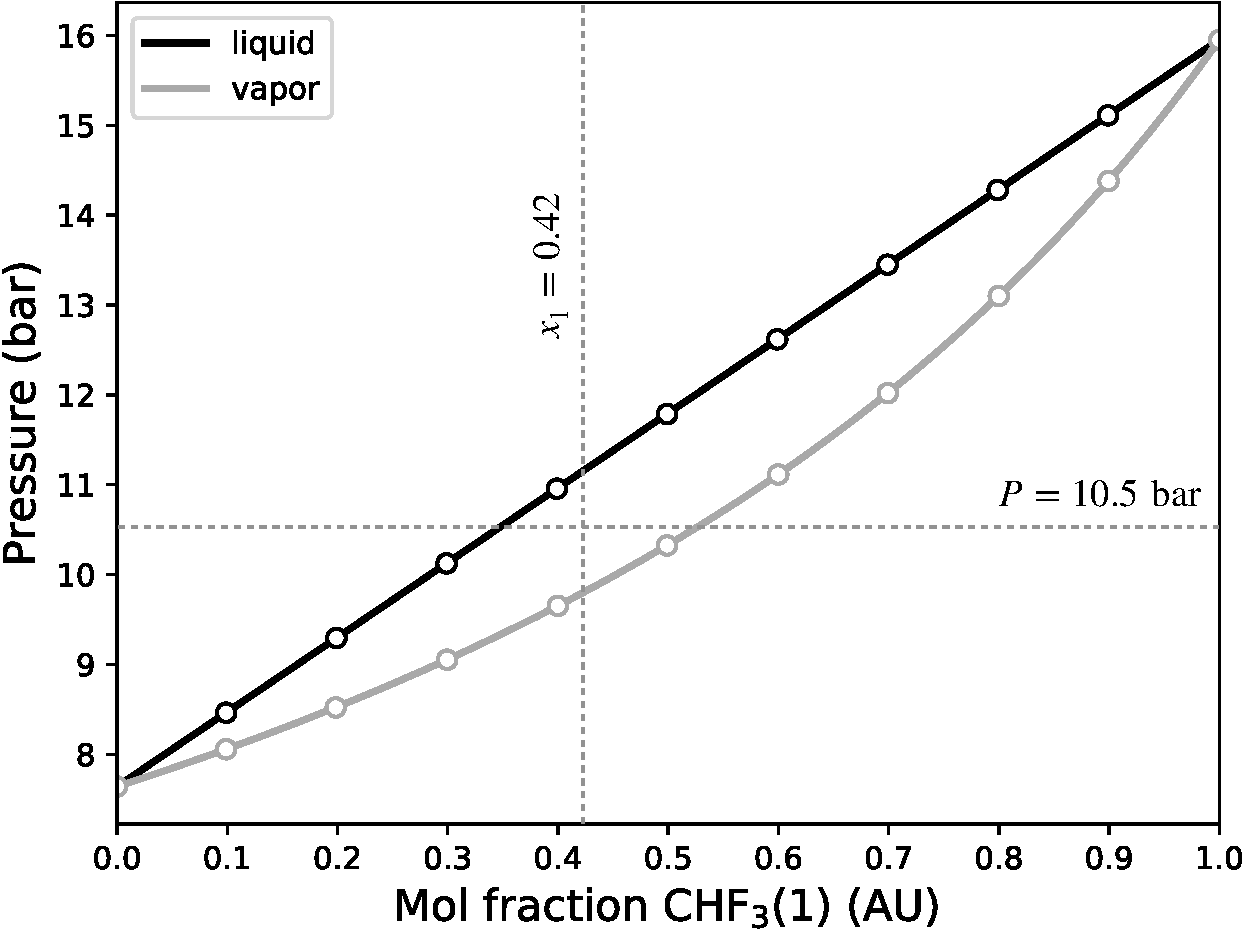
\includegraphics[width=0.75\textwidth]{./figs/VLE-Ideal-Pxy-P2-F19.pdf}
    \caption{Pressure (bar) versus composition (x$_{1}$ and y$_{1}$) for a binary mixture of CHF$_{\mathrm{3}}$(1)/C$_{\mathrm{2}}$F$_{\mathrm{6}}$(2) computed assuming ideal liquid and vapor phases.}\label{fig-VLE-ideal-problem}
    \end{figure*}
    
    \item{(XX points) Cornell Inc. was hired to design a flash separation process for a binary ($\mathcal{M}$ = 2) mixture of CHF$_{\mathrm{3}}$(1)/C$_{\mathrm{2}}$F$_{\mathrm{6}}$(2).
    The engineering team performed initial design calculations using Raoult's law for z$_{1}$ = 0.42
    (Fig. \ref{fig-VLE-ideal-problem}). Let the saturation pressure of component $i$ be described by the
    Antoine equation:
    \begin{equation}
      \log_{10}\left(P_{i}^{sat}~[\mathrm{bar}]\right) = A - \frac{B}{C+T[K]}
    \end{equation}where the Antoine parameters are given by:
    
    \begin{table}[!ht]
      \centering
      \caption{Antoine parameters for the Flash problem.}
      \setlength{\tabcolsep}{18pt}
      \begin{tabular}{c|c|c|c}\toprule
        Species & A & B & C \\ \toprule
        CHF$_{\mathrm{3}}$ & 4.45 & 718.1 & -22.01 \\
        C$_{\mathrm{2}}$F$_{\mathrm{6}}$ & 3.980 & 677.1 & -24.51 \\\bottomrule
      \end{tabular}
    \end{table}
    
    \textbf{Assumptions}: (i) the Flash drum operates at steady-state;
    (ii) vapor-liquid equilibrium occurs everywhere inside the drum at some (T,P);
    (iii) treat both the vapor and liquid phases as ideal;
    (iv) the Flash drum is well-mixed;
    (v) a single liquid feed (stream 1) enters, and a vapor (stream 2) and liquid (stream 3) exit the drum;
    (vi) R = 8.314$\times$10$^{-2}$ L bar K$^{-1}$ mol$^{-1}$.
    
    \begin{itemize}
      \item[a)]{(XX points)~What temperature T (K) is the Flash drum operating at? (place your estimated T in Table
      \ref{tbl-state-flash-problem}).}
      \item[b)]{(XX points)~\textit{Graphically} estimate the mising values in Table \ref{tbl-state-flash-problem} assuming the Flash drum operates at P = 10.5 bar with a input feed rate of $\dot{F}$ = 10 mol/t and $z_{1}$ = 0.42.}
      \item[c)]{(XX points)~\textit{Analytically} check the graphical estimates of $\dot{L}$ and $\dot{V}$ using the pressure summation expression:
      \begin{equation}
        \sum_{i\in\mathcal{M}}z_{i}\left[\frac{P_{i}^{sat}}{P}\left(\frac{\dot{V}}{\dot{F}}\right)+\frac{\dot{L}}{\dot{F}}\right]^{-1} = 1
      \end{equation} If this expression is \textit{significantly} different than 1 (greater than $\pm$~10\% difference),
      please re-estimate your values (show your work).}
    \end{itemize}
    
    \clearpage
    
    \begin{table}[!ht]
      \centering
      \caption{State table for the Flash problem.}\label{tbl-state-flash-problem}
      \renewcommand{\arraystretch}{2.0}
      \setlength{\tabcolsep}{18pt}
      \begin{tabular}{c|c|c|c|c|c|c}\toprule
      Stream & State & T (K) & $\dot{n}_{s,T}$ (mol/t) & $x_{1}$ or $y_{1}$ & $x_{2}$ or $y_{2}$ & P (bar) \\ \toprule
      1 & L & N/A & 10 & 0.42 & 0.58 & N/A \\ \hline
      2 & V & & & & &  \\ \hline
      3 & L & & & & &  \\ \bottomrule
      \end{tabular}
    \end{table}}